
\chapter{Exploration 4: creating the necessary requirements to measure the frustration of users in XIMPEL}
% Question: how do we extend XIMPEL with data logging? What theoretical knowledge do we need to analyze the quality of experience, engagement and frustration?

At one point while I was playing with XIMPEL I noticed that I found it to be a shame that every playthrough would be forgotten after it had ended. I wanted some form of memory. I wanted some form of logging. I then realized that creating a logging framework and creating a theoretical framework on how to measure frustration with it would be valuable for improving the user experience of XIMPEL. So in this exploration I am finding out what kind of theoretical framework for frustration (and to a lesser extent engagement) we should have and from that framework what the minimal requirements are regarding data capture.

One reason I chose frustration as an important metric for user experience is because it seems that the experience of frustration is still quite misunderstood in academia. Having written earlier about frustration from a psycho-neurobiological perspective, I had the idea that I would be most productive for the academic community if I would resume my work in this area of research. Another reason is: this is my first attempt and experience at answering an artificial intelligence question while having a background in it through other disciplines, which is exciting!


% Why do I start to talk about my measures first and *then* have a literature review?
% Ik laat ook niet de wetenschap zien achter facial expression detection

\section{Justification for creating a logging framework}
% Tell here that you created history graphs and what it is useful for
One justification is: to understand your users. Hugo Huurdeman shows this justification in work that happened at more or less the same time \cite{ximpel_norway_first_article}. In order to understand more about the user experience (UX) that XIMPEL users go through I have created the beginning of a framework that logs data needed for classifying frustration or engagement. Understanding whether a user is engaged or frustrated helps to improve the UX for authors creating XIMPEL presentations. I chose for frustration and engagement because it will give insight into whether a user wants to quit in the middle of a XIMPEL presentation (frustration) or is driven to see all of it (engagement). Moreover, it begs the question: how does one measure and classify frustration and engagement in hypermedia frameworks? For this question I emphasize a focus on frustration, because quitting an application out of frustration is a more urgent problem to solve than to keep users fully engaged. Another question that came up is: does frustration always lead to quitting behavior? The answer to that is no it does not always lead to quitting \cite{roest2015}. A follow-up question would then be: is it possible to differentiate between different frustrations? To which I found a tentative slightly surprising answer by accident.

Since hypermedia frameworks are interactive they have on some dimensions more in common with digital games than with multimedia. A single video does not allow for much interactivity. However, with XIMPEL it is possible to create a point and click adventure game. Therefore, I chose to review the literature on engagement and frustration regarding digital games. A second motivation to do this is because XIMPEL is an intentional intersection between hypermedia and gaming.

My approach for reviewing this literature is as follows: I draw from my own previous literature review, written in 2015 about what frustration and engagement is and add to that review with new research findings. I furthermore, review literature on how engagement but most notably frustration are measured and classified. 
The result of this literature review will influence my choice of measures that I will include in creating a logging framework for XIMPEL. Furthermore, these measures will have a focus on accessible non-customized hardware, which means conventional hardware available on most laptops and tables. Another result is a literature review itself, which is guided for design and not for comprehensive review but because of that an example of bridging literature to implementation.

\section{What is frustration}
% Check to see if there are new articles, otherwise just take stuff from your old thesis.

In gaming, to frustrate a player means to block their progress. Or as Gilleade and Dix state it, it is: ``that which arises when the progress a user is making towards achieving a given goal is
impeded.'' \cite{gilleade2004} In general, players will feel frustrated when they realize that the blocking of their progress has happened. 

% generality of the definition?
Despite that this definition has been made in a gaming context, it seems to be quite general. Studies about completely different topics (e.g. human motivation) give very similar definitions, albeit implicit. Take for example (emphasis by me): ``Recently, it has further been recognized that beyond measuring need satisfaction versus the lack thereof, needs can also be \textit{actively blocked} or the growth potential of individuals, \textit{the frustration of these needs} would elicit defensiveness, ill-being, and even psychopathology.'' \cite{chen2015} Because of this generality, the definition of Gilleade and Dix will be used.

% Probably not include this, but leave it here for an interesting comment: Frustration can refer to no or little progress in achieving goals due to limited skills and strenuous challenges in tasks -- definition of Csikszentmihalyi 1988

% the nuances of frustration
\subsection{Some nuances regarding frustration}
It matters to whom or what the frustration is attributed to. If the frustration is attributed to oneself it will not cause quitting a game. If, however, it is attributed to the game itself (e.g. lag or too difficult AI) or to another person (e.g. the co-player did not perform well in a task) then the player will quit. This is indeed a quite subjective experience. More forgiving players might attribute the frustration more to themselves than to their co-player, for example. In my literature review, I provided some evidence for this claim but the strongest evidence for it has been found in a recent 2017 study about near-misses in Candy Crush.

The near-miss is a form of frustration where attribution of a failure, which was almost a success, is attributed to oneself. The canonical example of a near-miss is a slot machine that almost shows three lucky number sevens, but the third seven goes a little but too far and reaches over the line, leaving itself at the right bottom corner of the slot machine (see figure \ref{fig:near_miss}). 

\begin{figure}
    \centering
    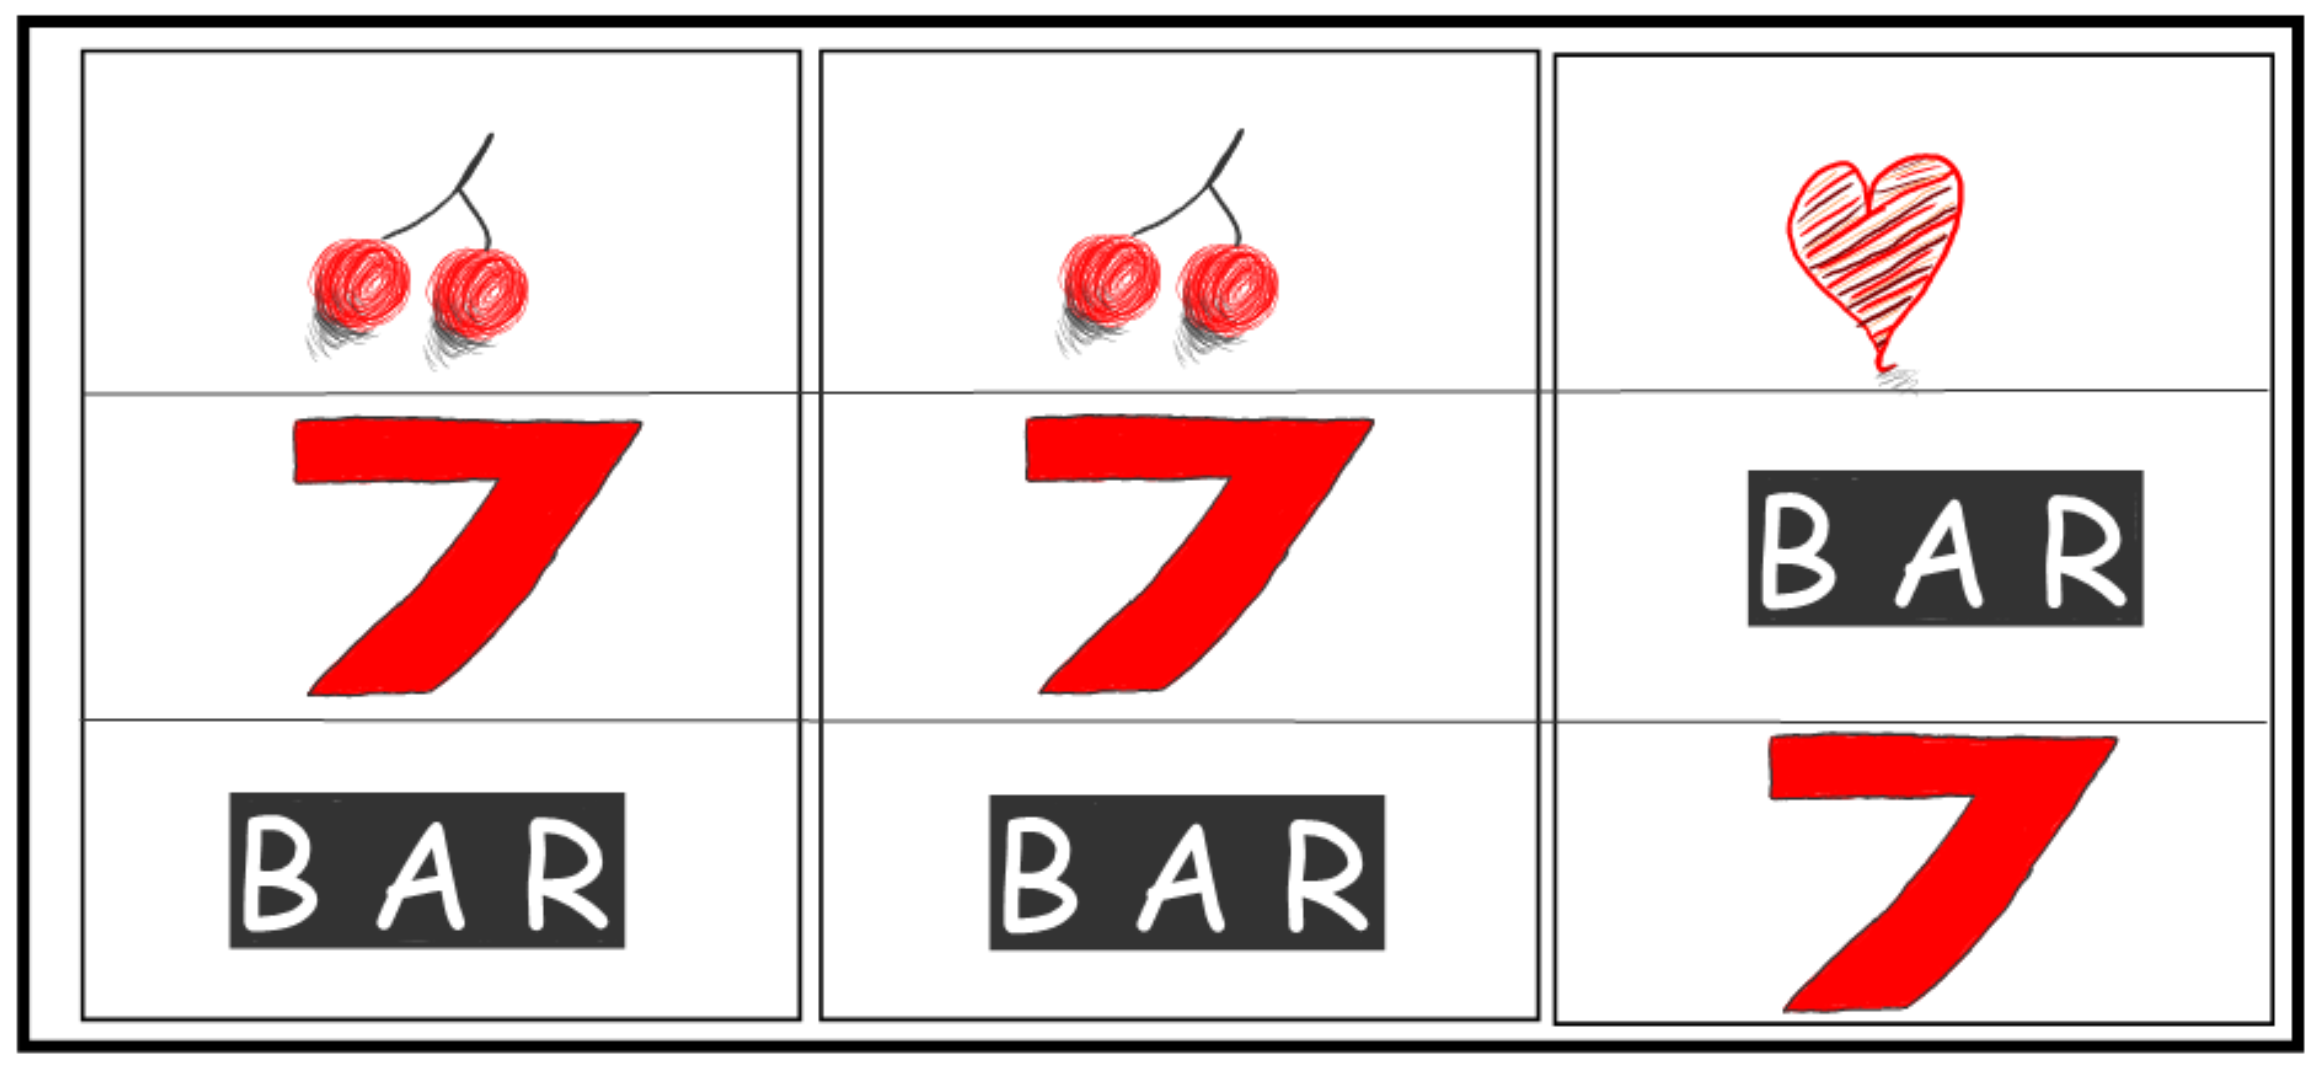
\includegraphics[width=1.35\textwidth, center]{near_miss.png} % quotation marks make sure file name does not display
    \caption{A visual example of a near-miss. The lucky number 7 on the third slot machine column went one place further than intended.}
    \label{fig:near_miss}
\end{figure}

In the study, researchers found that the near-misses in Candy Crush increase the wanting to play and frustration \cite{larche2017}. This is clear evidence for the idea that the attribution of frustration matters since players believe they are able to achieve their goal. For XIMPEL authors understanding this distinction is important when their application resembles a game.

However, when the XIMPEL application resembles multimedia more in the sense of that it is a XIMPEL application in which the user is passive, then the attribution of frustration is in almost all cases on the XIMPEL application itself. When a user is passive, he or she cannot do much in the first place and will therefore most likely place the blame on the application. That blame may be placed on several factors such as: topic mismatch, badly designed applications, the XIMPEL control buttons, or a terrible quality of experience (when watching YouTube videos or other networked media types).

XIMPEL authors need to consider to what extent they deem frustration and the willingness to quit important. In some contexts, frustration matters less. For example, when students are made to watch any presentation during their student lifetime at university, frustration will only lead to disengagement but not to quitting. One might think that this is just as bad, but one study shows this is not always the case. 

Computer scientists at the University of Saskatchewa in Canada created a game to create interpersonal trust in which they showcase: a literature review on what interpersonal trust is, a literature review on how it is developed in real-life and via digital games and an experiment if their game fosters trust. The interesting result is that their game was found to be frustrating. They remark:  ``Our game was strongly affected by networking issues, which made the game more frustrating and difficult than we expected. ... participants in the game condition scored low on competence and high on tension. Comments from the debrief as well as the recordings of the game session confirm that many participants experienced a frustrating, `buggy' game, rather than the playful experience we intended.'' \cite{depping2016} They also state that this situation caused the game to become an out-group and the players to become an in-group, which fosters trust\footnote{I will skim over the fact that they implied on some level that a game is a person (an out-group in this case). Media like games, are social things that we project human values on. Unfortunately, I know too little to academically defend this position and will defer to my media studies and other social science colleagues. These types of things should be discussed more often in computer science literature in order to have stronger assumptions and assertions.}. A game does not have to be fun to reach its designed goal \cite{depping2016}. It could even be very frustrating, it could even be a negative experience. 

% \section{What is engagement}
% % Check to see if there are new articles, otherwise just take stuff from your old thesis.

% % I need to make quite a strong note somewhere on the relationship between frustration and engagement and how it is under
% % https://link-springer-com.vu-nl.idm.oclc.org/article/10.1007/s40429-017-0163-x -- children's motivation to play video games

% https://www.semanticscholar.org/paper/Predicting-User-Engagement-with-Direct-Displays-Us-Arapakis-Leiva/50b73a320e600b841be0bde76be562ac18ca1674 -- maybe check that out for classifying engagement -- all kinds of mouse metrics for measuring engagement and frustration

% Recently an updated literature review about the impacts and outcomes computer games have (2016) has shown more insights into what engagement is \cite{boyle2016} (the older systemic literature review was from 2012 \cite{connolly2012}). In the timeframe of four years, 22 studies done on engagement were deemed acceptable enough for the reviewers. It paints a clear picture how researchers are defining engagement in different ways and some researchers try to move away from the flow theory first formulated by Mihaly Csikszentmihalyi \cite{boyle2016}. 

% The most compelling 


\section{Capturing data for analyzing frustration}
% Just write out and justify what you've created and what is too hard because of time-constraints. Do technically explain how facial expressions get measured.
% Explain here that you could do studies such as correlating facial expressions with mouse movements

Since XIMPEL is a framework with the browser in mind, I have assumed that most users only have access to standardized hardware. This is because at this moment XIMPEL is used by students at the Vrije Universiteit Amsterdam and by organizations who use it in giant tablet installations. Because of time-constraints I used measures that I could only find on my MacBook Pro (2015), since that is the hardware available to me. 

This constraint takes precedence over evaluating academic literature. No organization has given me the tools to do something else and I do not have the funds available to buy specialized hardware. However, some of the reviewed literature (see the next section) does use specialized hardware. Despite this mismatch, these articles provided inspiration nonetheless on the nature of frustration, measuring it or classifying it.

\subsection{Frustration measures: clicks, mouse speed, user XIMPEL subject history and facial expressions}
XIMPEL users tap or click on overlays, which means that taps (not available on my MacBook Pro) or mouse clicks need to be measures. Furthermore, measuring mouse moves at the exact moment when they are made allows for the inference of acceleration or deceleration of the mouse and some estimated average speed in general. Since XIMPEL developers also know on which x and y coordinates their overlays are, they can also analyze through the mouse position if the user is standing on an overlay or media item.

Finally, measuring the starting time and which subjects the users are in at any moment allows for the construction of a path where users have been and for how long. This used to be in the old XIMPEL framework (written in ActionScript) but has not yet been implemented when it was ported to JavaScript.

Measuring: mouse clicks (x, y and time), mouse moves (x, y and time), starting time of playback per subject (in milliseconds) and the subject ID forms the basis of measuring frustration. It is quite unfortunate that these measures are relatively indirect. Frustration is a feeling first and foremost and gets expressed through the user in a variety of ways. 

The need to obtain more direct data was there since these measures are perhaps too indirect to be useful for classifying frustration. Maybe it would be possible to capture frustration through the use of a web cam. While it is not as standardized (or unobtrusive) it may help greatly in the situations in which it can be used. So I decided to make that an optional measure. Sending web cam data directly is a lot of data to store. Therefore, I decided to classify facial expressions directly through the CLMtrackr JavaScript library. It detects: joy, anger, surprise and sadness. It has to be noted that this is a trade-off to make. Does a data capturing server store video streams or does it store classified data? The disadvantage of the former is that there is a lot of data to store, the disadvantage of the latter is that the data contains less information since there is a lot more one can do with pure video data than classified facial expressions. How this classification works is explained later in the chapter. 

The use of CLMtrackr and classifying emotions related to frustration have two reasons. (1) Detecting facial expressions in the browser in general is difficult, so it is better to work with libraries already in place for this. As of writing, this is the only library I came across. And (2) in the reviewed literature on facial expressions (see section \ref{frustration_facial_expression_literature}), there is a strong argument to be made to not measure the facial expression of frustration. To summarize (2): the detection of anger may be useful since frustration and anger are very related through the frustration-aggression hypothesis \cite{roest2015}. Sadness may be useful as well since it can be caused by a hopeless variant of frustration \cite{kuppens2003}.

\subsection{Software architecture and implementation for capturing data}
% Client-server and stored in a database
% Have some screenshots
% Discussion point here: there is double work done on the server-side of things

All the mouse click, mouse moves, starting time, subject ID and classified facial expressions are sent to a NodeJS server. That server created a session ID to the client beforehand (including the date and the time) and stores everything in a postgres database. The data stored can later be retrieved for classification. The reason for not doing it on the fly is because it is computationally expensive and perhaps even wasteful. The detection of frustration is only relevant when developers want to improve the UX of XIMPEL. NodeJS with Express has been used because developing with an unopinionated microframework allows for the quick creation of routes that stores data in a database. The data can be queried from the database using any kind of program. 

Independent parallel work has been done in similar fashion by the programmers of the University of Oslo who develop XIMPEL applications specifically for tablets. Instead of using NodeJS and Express, Python was used in combination with Flask, which leads to a more or less similar communication pattern between XIMPEL and the server-side data capture application \cite{ximpel_norway_datacapture_server}. 

% to do -- maak plaatje hiervoor -- maybe

% Measures
% Facial expressions (angry, sad, happy, surprised)
% Mouse clicks (x, y)
% Mouse moves (x, y)
% Starting Time
% Subject Id

\section{Classifying the measures as frustration} %think about this
% Before you start your own thoughts, look up literature first

Now that we have a way of measuring raw data for frustration, the next question is: how to determine when a user is frustrated with this data? The approach for this is to first look at previous research and then conceptualize a possible classification method.

% It is around this time that I started to ask myself if there had been research on this. And to my surprise there was! This comes as a surprise since the literature on a nuanced view of frustration is rather sparse. So I believed there would not be research that would classify frustration. I was wrong. So while I did already determine my metrics on how to measure frustration, it is only now that I started to read about others who did the same.

I do need to note that I did not implement a classification algorithm. It is outside of the scope of this project to implement it. However, conceptualizing a first iteration of such an algorithm or algorithm design approach leaves opportunity for further realization in future work.

\subsection{Related Literature}

% input --> AV-space --> emotions
% Do I need images or diagrams for this?
\textbf{Depping, Mandryk, Johanson, Bowey and Thomson} used four inputs (galvanic skin response, heart rate and EMG frowning and EMG smiling) in order to calculate arousal and valence values. A certain combination of arousal and valence (which is a range from displeasure to pleasure) would yield a particular emotional state: boredom, challenge, excitement, frustration, and fun. Each input is a time series that would be used to create a time series for arousal and valence, called AV-space (figure 1, 3, 14 and 15 in their paper \cite{mandryk2007}). 

For example, increasing galvanic skin response would be mapped to increasing arousal. Low or high galvanic skin response would be modulated with heart rate data, where a low heart rate would result with a lower arousal level than high heart rate data. EMG Smiling would mean that valence levels increased and EMG frowning would mean that valence decreased. They had other rules which have been written in more detail in \cite{mandryk2007}.

Then, they created a mapping from AV-space to emotions. In particular, frustration needs to have a high arousal (e.g. high galvanic skin response and high heart rate) and low to medium valence (i.e. displeasure, e.g. frowning on the EMG). They discuss all their emotional states in their paper \cite{mandryk2006} and go into more detail in another paper \cite{mandryk2007}. Through a user study they found that their predicted model of frustration did not coincide with self-reported frustration. This was not the case with for the emotions fun and excitement \cite{mandryk2006}.

% Picture would be nice, since it makes it easier to understand

% Cogni Mouse
\textbf{Researchers in Cyprus and Portugal}\footnote{To make it a little bit confusing, one of the researchers is called David Portugal. His last name and the name of the country Portugal bear no affiliation. Jo\˜ao Quintas is the researcher who is affiliated to a Portuguese laboratory.}, created a new mouse called CogniMouse\cite{portugal2016} for older computer users. With this mouse they hoped to measure frustration since some older computer users have some difficulties using computers at work. While I am not developing my own computer mouse, it is interesting to see which extra measures the research team was trying to get. The sensors in the mouse are a: ``galvanic skin response sensor, temperature sensor, inertial measurement unit (IMU), grip/pressure sensor, and heart rate sensor.'' \cite{portugal2016} They used a classification algorithm that employs ``Bayesian-based formalism inspired on conditional probability distributions.'' \cite{portugal2016} This means that they used a formula that constantly calculated a probability to what extent the user was frustrated. They used: grip force, acceleration vector and click stream frequency as inputs. The formula itself is:

$$P(Frus|Grip,Acc,Click)=\dfrac{P(Frus)*P(Grip|Frus)*P(Acc|Frus)*P(Click|Frus)}{P(Grip)*P(Acc)*P(Click)}\cite{portugal2016}$$

The formula clearly shows the Bayesian nature of the classifier. They have a planned user study and present a use case scenario of a middle aged woman who would experience issues using a new computer system. The CogniMouse noticed her frustration and helped her by presenting a graphical help wizard. In their future work they will add more ways to track the user, such as an eye tracker.

% measuring frustration in keylogs in a programming course
% using bayes method to detect frustration with keystrokes, mouse strokes and interaction logs
\textbf{In the study of \cite{leong2016}} an annotator annotated the signs of frustration from web cam recordings, where students in those recordings made use of web based programming tutoring meant for a Java programming course for beginners within University of Singapore. Students mouse clicks, keystrokes and actions were written into log files. This was compared to the annotations on a time scale. After this comparison, relevant extracted metrics were: ``the mean and median key latencies, number of keys, wait time (duration longer than 1 second with no key inputs), back space and delete key latency and frequencies and the frequencies of mouse clicks. The interaction features include the number of compilations, number of errors encountered, number of exercises completed and the duration of time spent working on the exercises.'' \cite{leong2016}

The extracted features were aggregated into a sliding window with sizes of 30, 60, 90, 120, 150 and 180 seconds; where windows would overlap each other for one-third of whatever window size was determined. Frustration would be observed per sliding window. If the frustration occurred in the overlapping sliding window part, then both sliding windows were annotated as a frustrating event. Changing the window width from 30 seconds to a 180 seconds -- and everything in between -- would have consequences for the detection of frustration. If someone gets frustrated within every 3 minutes, then a window size at the highest width would always be marked as frustrating, this would not be the case for lower window width sizes. The problem with lower window width sizes is that there might be insufficient data to determine anything at all.

To classify frustration within these sliding windows they trained a Bayesian network and compared it to a naive Bayes model. The performance of the Bayesian network compared to the naive Bayes model was a significant improvement. The performance improvements were 32.79\% (under the curve, they authors did not define what this means), 32.73\% (accuracy, ``the number of correctly identified instances divided by the total number of instances'' \cite{leong2016}) and 2.53\% (sensitivity which ``measures the true positive rate or the proportion of positives that are correctly identified as such while specificity measures the proportion of negatives that are correctly identified as such'' \cite{leong2016}).

% Stress on e-learning students
\textbf{Instead of classifying frustration, one could also classify something else such as stress}. Rodrigues, Gon{\c{c}}alves, Carneiro, Novais and Fdez-Riverola did this \cite{rodrigues2013} in a study for which they created a stress detection tool in for the e-learning platform Moodle. They created a system called the Dynamic Student Assessment Module (DSAM) which has all kinds of components for detecting the mood of a student. The DSAM does this in two ways: by asking students through a questionnaire and by looking at their behavior. They looked at their behavior through ``facial analysis, mouse analysis, keyboard analysis, and log analysis (through Moodle logs).\cite{rodrigues2013}'' The features they analyze are: ``the number of mouse clicks per minute, the average duration of mouse clicks (from the button-down to the button-up event), the maximum, minimum and average mouse speeds, the keystroke rate (strokes per second), the average duration of a keystroke (from the key-down to the key-up event) and performance measurements.\cite{rodrigues2013}'' They asked 10 students to do two similar programming tasks. In one programming task they were stressed through the use of a time limit and being told that this assignment was very important for their future (academic) career.   They found that the following JavaScript events were fired a lot more when students were stressed: key down, key up, mouse down, mouse up, mouse wheel and mouse movement. In some cases it was 5 times as high, in other cases about 1.5 times as high. From these differences they claim they can detect stress.

\subsection{Proposed approach for classifying frustration in XIMPEL}
In the related work section a lot of input sources have been described (too many to list). Classification techniques were: rule-based, Bayesian and comparing it to a control group. Furthermore, \cite{mandryk2006} wrote about another author using Markov chains. It seems to be the case that any probabilistic classification technique can be tried. Other than probabilistic classification techniques, rule-based techniques sometimes seem to work -- comparing results to a control group is a specific example of a rule-based technique.

In XIMPEL we measure: mouse clicks, mouse moves, a historical trail (with time) of which subjects a user goes to and facial expressions. Since a hypermedia-like application could be different than a game or a generic application due to watching video, some measurements will not always be the same. For example, someone could get frustrated at miss-clicking on an overlay, finally the user will click on the overlay. Compared to a non-frustrated user, the frustrated user will likely have more clicks. But if a user is frustrated because a certain video is boring and he or she cannot go to the next subject, the frustration may only show via their facial expression and not through their use of how they use the computer mouse.

Since it seems more important to give insight to XIMPEL authors when a user is \textit{possibly} frustrated, I put more emphasis on detecting all true positives. In order to detect all true positives, one must be willing to accept that there will be possible false positives. In order to get all true positives one must minimize false negative occurrences of frustration and thus be forced to have more false positives. At the same time, looking into a particular possible frustrating episode must be worthwhile so having a signal to noise ratio of 10 to 1 might be a bit much since it might take 2 to 5 minutes to check a possible occurrence of frustration (e.g. checking the data for a particular person for a possible frustrating occurrence). A signal to noise ratio of 1 to 3 would be much more acceptable. For example, if the signal to noise ratio is 1 to 3, then it would take 20 minutes at worst to look at instances of possible frustration.

So the requirements for our classifier are:
\begin{itemize}  
    \item A signal to noise ratio of 1 to 3 or lower (specificity).
    \item If the first requirement is not broken yet, then get more, or even all, occurrences of frustration (recall).
    \item Be able to pickup on frustration when the user is not using computer peripherals (e.g. listening to audio or watching a video).
    \item Be able to pickup on frustration when the user is using computer peripherals.
\end{itemize}

Time constraints prevent me to create such a classifier. Nevertheless, I will write my ideas down for future work related purposes. Since interactive video, hypermedia and XIMPEL applications are a bit different than other applications, an observation study should be done as to what makes users frustrated. From such an observation study it should be possible to see what frustrated behaviors users have and how this could be possibly measured. The measures that I programmed for are a mix of a best guess inspired by literature and hardware constraints.

Classification should depend on the requirements for detecting frustration within XIMPEL. These requirements are listed above and were made with the rationale of why we should detect user frustration within XIMPEL applications in the first place which is to improve UX. The requirements are fairly broad, which means that a potential solution does not have to be perfect. It is likely that multiple solutions are possible.

My approach to classifying frustration would be to create a simple classifier per input type. So there is a mouse movement frustration classifier, for example, and also a facial expression frustration classifier. If one of these classifiers gives an alert, then frustration is possibly detected. This is possibly too straightforward, but it allows to get more experience as to which input types explain frustration independently from the other input types. Testing which classifiers give too many false positives is future work. The question that I will attempt to answer now is how does each classifier work?

While this is one question and directly applies to mouse clicks, mouse moves, user trials and time between subjects; it applies differently to detecting frustration in facial expressions. CLMtrackr already classifies facial expressions. So the question regarding facial expressions goes much deeper and this depth is written down. Then, I realized that in my first literature search on detecting frustration in users I did not find anything about how to detect frustration in facial expressions, so I did a separate literature search for that specific question. So the specific questions regarding frustration in facial expressions are: (1) how does the current classification algorithm work regarding basic emotions? (2) do classified basic emotions help classify frustration, if so, how? And (3) why not detect frustration as a facial expression directly? Perhaps noticeable, questions 2 and 3 are related to how does the facial expression classifier work?

\subsubsection{Facial expressions}
% Anger --> frustration
% Sad... ?
% Happy, surprise --> engagement
% Leg uit waarom je voor een proxy moet gaan
The JavaScript library CLMtrackr classifies anger, sadness, happiness and surprise and gives all four a value between 0 and 1. 
CLMtrackr does this through constrained local models (CLM) among other things. It technically also classifies contempt and fear but not good enough according to a quick discussion with the CLMtrackr author on the Github Issues page \cite{github_issue_clmtrackr}, which is why these facial expressions are not classified. CLMtrackr trained its facial recognition abilities through the MUCT Landmarked Face Database (MUCT: Millborrow -- the author -- University of Cape Town)\cite{milborrow2010}. This database has 76 points (called landmarks) annotated on 3755 faces. It is possible to see an example image of such an annotated face on their homepage \cite{milborrow2010}. 

What follows now is a high level explanation of how this works. However, the mathematics will not really be explained since they have been explained quite well in the online resource of \cite{auduno2014}, which I recommend to anyone interested in the technical details of facial detection. That article also points to amazing resources on CLM itself.
The algorithm that Clmtracker uses is called subspace constrained mean-shifts, which is a form of a CLM and is authored by \cite{saragih2009}. CLM algorithms in general have two strategies that happen iteratively until some optimum has been found as explained in \cite{saragih2009}. 

\begin{itemize}
    % \item 1. perform an exhaustive local search for each PDM landmark around their current esti- mate using some kind of feature detector
    % \item 2. optimize the PDM parameters such that the detection responses over all of its landmarks are jointly maximized.
    \item 1. Exhaustive local search: perform a local search for each landmark in the model around their current point estimate. Use a classifier that will generate a probability map and associate the landmark to the highest probability pixel on the map.
    \item 2. Optimization: it could be that some landmark to pixel associations are a bad fit because there were no high probability pixels on the map. Shift their point estimate to somewhere else by calculating where there are likely higher probabilities.
\end{itemize}

The mathematical techniques that make this possible are explained below. I do have to caution the reader that I intuitively understand what is happening, but I do not understand the mean-shift algorithm and associated algorithms well enough to explain its details. Such details can be read in \cite{saragih2009}. Furthermore, data cleaning techniques that are used are not presented at all in this thesis (see \cite{saragih2009}).

The author of CLMtrackr built a model through the use of Principal Component Analysis (PCA), which informally speaking is a method by summarizing as much variance into a component. This is done by first calculating the mean points of all the landmarks of all the annotated faces, then PCA is used to extract the variations as components (they can also be seen as linear combinations of vectors). PCA has the property that the first component accounts for the most variance, the second component for the second most variance and so on. This means that with a few components most variance has been accounted for. PCA is therefore really useful as a data summarizing technique. The components themselves are uncorrelated to each other\footnote{An in-depth mathematical student explanation on can be found on \url{http://www.cs.otago.ac.nz/cosc453/student_tutorials/principal_components.pdf}. The best visual explanation about PCA is to be found here: \url{http://setosa.io/ev/principal-component-analysis/}. The best visual explanation for eigenvectors is here: \url{http://setosa.io/ev/eigenvectors-and-eigenvalues/}.} The PCA model of a generalized face can be viewed at \cite{clmtrackr_model_viewer}. Playing with it gives a better intuitive understanding of what PCA does regarding finding the average model of a face and the variations of that on a per component basis. 

The model has 70 points. Each point in the model has been associated to one classifier during training, meaning there are 70 classifiers for the model in total. Each classifier has been trained by cropping a small patch of its associated annotated point per facial image (3755 facial patches per annotated point in total). The classifier for such a patch is a logistic regression classifier with a support vector machine linear kernel (and a MOSSE filter which is of less importance). The reason it is a logistic classifier with a linear kernel\footnote{The author Audun Mathias Øygard calls it an SVM kernel. However, digging into the source code it seems that the so-called SVM kernel is a linear kernel. I had to dig deeper since there is no such thing as an SVM kernel. The kernel can be seen here with a search query in the Github repository: \url{https://github.com/auduno/clmtools/search?utf8=\%E2\%9C\%93&q=kernel}} is because it ``is what the original paper suggests.'' \cite{auduno2014}

\textbf{Exhaustive local search.} When the classifiers are used it crops a local (i.e. small) search rectangle around its initial position and calculates a probability map of pixels which are aligned with the landmark. When this works, such a map has a few high probabilities lying around in the center, of which one of them is the highest and that pixel value (or grid of pixels) will be associated to the landmark. This is done for all 70 landmarks in the model. 

\textbf{Optimization.} However, doing this there is one problem. Since the local rectangle might be too local. The problem with this is that some classifiers cast their local rectangle in a different area compared to where the actual facial feature is (e.g. an eye). In order to counter this, a second step is being done that is akin to gradient descent. This is done by shifting the point of a landmark, which means when it will cast a new rectangle to search for the highest probability it will find new values. The method is called a mean-shift. This mean-shift is determined by using expectation-maximization.

By doing all of this we have found faces. What we have not found are facial expressions. These are classified using logistic regression. The parameters of the facial model are used as features. To get training data for the regression, images of people expressing emotions have been annotated and projected on the PCA decomposition. By doing this, the closest parametrization is achieved. What is not done but could be done for future work is to first determine a neutral baseline, since it is not clear how expressive emotional faces are beforehand. The emotion classifier can also be viewed since the regression coefficients can be used as parameters for the facial model. You can view it at \cite{auduno2014b}.

\subsubsection{Detecting frustration through CLMtrackr}
The facial expression of anger is interpreted as frustration. The facial expressions of happiness and surprise is interpreted as its opposite: engagement. Sadness might be a meaningful measure of frustration as well since it has shown to correlate as much to frustration as anger \cite{kuppens2003}.

It is important to keep the classification of engagement since it may give extra data if another classifier does classify that the user is frustrated. In most cases facial expressions should take precedence over mouse clicks, mouse moves and history graphs because a facial expression conveys how a user feels, much more so than the other measurements. The reason for that is that facial expressions are much more connected to emotions than the other units of measurements since facial expressions are a display of emotions.

% Not included in this thesis:
% https://www.paulekman.com/blog/anger-problem/
%% Reason: blog post and no sources

% https://www.paulekman.com/blog/respectful-disagreements/
%% Reason: blog post and no sources

% https://journals.lww.com/nursingresearchonline/Abstract/2010/05000/A_Meta_Analytic_Study_of_Predictors_of_Anger_in.4.aspx
%% Reason: I'm lazy, site does not load and I need to get this done

% ---

It may seem a bit of a cop out to use anger and sadness as a proxy of frustration. However, perhaps it is not. Anger is the result of a particular frustration. When a user is frustrated at anything other than him or herself, he or she will become angry \cite{roest2015}. Therefore, the detection of anger is a possible detection of frustration. Other research (not included in the literature review) that point to this direction is research about consumer anger \cite{funches2011}. The authors do not explicitly write about frustration, but in this study all the sub-categories of anger are related to frustration in the conceptual sense, they are: broken promises, unfairness and expressed hostility (by service employees to customers). Neuroscientific research shows that ``poorly controlled frustration, manifested as exaggerated anger.'' \cite{yamagishi2012} Research on emotion regulation implies the same, in one paper it is stated that ``a low frustration tolerance is related to trait anger and a higher level of frustration tolerance is related to lower levels of anger and longer persistence on difficult tasks.'' \cite{szasz2011} 

Kuppens, van Mechelen, Smits and de Boeck gave strong nuances to this view. In their article the appraisal basis of anger was evaluated to which components were necessary and sufficient. The researchers conducted two studies and they found that ``other accountability and arrogant entitlement, as instance of unfairness, are specific appraisals for anger.'' \cite{kuppens2003} They suggest that frustration and having an antagonistic action tendency co-occurs. This is easier to believe for having an antagonistic action tendency, since only one study found an association with anger. However, the reason they state for the feeling frustration leaves much to be desired. They studied the \textit{feeling} of frustration in their first study and \textit{goal blocking} in their second study. They found that goal blocking is not associated with anger but feeling frustrated is. They also found that feeling frustrated is associated with sadness \cite{kuppens2003}.

Putting anger and sadness side by side from their first study, it is observed that sadness has frustration as an appraisal-action tendency component and did not have any significant correlation with the other appraisal-action tendencies. Interpreting these results it could mean that sadness occurs when one feels hopeless because of frustration. Whereas if one feels angry because of frustration it is because of someone (or perhaps something) else. 

The result of Peter Kuppens et al. give an indication that indicators on sadness may be important as well. Therefore, the final conclusion of detecting frustration in facial expressions is that sadness and anger combined are an interesting proxy for frustration and joy and hope for engagement.

\subsubsection{Detecting the facial expression of frustration}
\label{frustration_facial_expression_literature}
The complexity of writing a thesis while programming is that a program can become obsolete when new literature is found. It is quite possible for a researcher to believe they are up to date for a certain topic, only to discover there was extra information out there available by a slight alteration of their search queries which they had not considered. This arguably happened for this project, or perhaps not. Indeed, an exploratory thesis such as this one is quite prone to requirements creep. Additional found literature seemed to answer one particular question: how does one detect the facial expression of frustration directly?

The following articles have not been found initially, because the importance of detecting facial expressions at all -- on a practical level -- had more importance. Both studies used the Facial Action Coding System (FACS) which divides the face up in certain sections. These sections are called action units. Humans code these action units on a 1 to 5 point scale in terms intensity. These 5 points are labeled as: (1) trace, (2) slight, (3) marked or pronounced, (4) severe, (5) maximum. Other modifiers are R and L which convey information that assymetrical movements happen on the right or left side of the face. 

In one article action units (AUs): 1, 2 and 14 (14 is of secondary importance) were associated with frustration. AUs are respectively named after their movements. For example, AU 1 is called the inner brow raiser, AU 2 is called the outer brow raiser and AU 14 is called the dimpler. Moreover, action unit 1 and 2 often occured together and ``triggered each other'' \cite{craig2008} which means that ``a raised inner brow tends to trigger a raised outer brow, and vice versa.'' \cite{craig2008}

An article written five years later (in 2013) compared the results of the authors of \cite{craig2008}, though not specifically from the paper that is outlined in the previous paragraph but a paper written by the same authors a year later \cite{craig2009}, which describes two studies one of them being the study of \cite{craig2008}. They found completely different results since they noted that frustration has a strong association with AU 4. They note that AU 1 was associated with whether a student self-reported their tutoring session (with JavaTutor) to be worthwhile. AU 2 was associated with whether a student self-reported the feeling of being rushed during a tutoring session. AU 14 was was associated with whether a student self-reported with whether how successful he or she felt in the accomplishment of a task. All the AUs they found for their dependent variables were: AU 1, AU 2, AU 4, AU 7 and AU 14. They measured self-reported frustration as: ``How insecure, discouraged, irritated, stressed and annoyed were you?'' \cite{grafsgaard2013} It could be the case that they measured something different than frustration since: ``discouraged, irritated, stressed and annoyed'' is not particular to only frustration, whereas the other questions in their post-session survey seem to be related to frustration. The authors note a similarity with how they detected AU: 1, 2 and 14; with its relationship to frustration in previous research as well. They seem to suggest that these action units are related to frustration. Finally, their research shows how difficult it is to replicate previous research in this area.

This difficulty is also seen in the final article found for this section, which has been peer-reviewed but will be published later in 2018. The topic of research was detecting frustration in frustrated drivers. In this study the authors found that they were mostly in line with the action units that also have been found by Ekman, which are AU: 4, 14, 23 and 24 \cite{ihme2018}. These action units are only partially in line with research from the previous paragraphs written. The authors from the previous paragraphs found evidence for AU: 1, 2 and 14 \cite{craig2008, grafsgaard2013}. The authors of \cite{ihme2018} note that these action units have been linked to other emotions such as surprise (AU 1 and AU 2)\cite{ihme2018}. In their final results they found no significant result for AU 4 and AU 14. They did find a significant result for the association of AU 23 and frustration. They also did find a significant result for the association of AU 24 and frustration. They furthermore did an exploratory analysis, meaning they also looked between a difference of their control condition and experimental condition while considering all the other action units. In this analysis they found that AU: 10, 12, 17 and 20 also had significant differences between the experimental and control condition.

It could be that frustrated driving does not capture the same type of frustration as a facial expression compared to computer-mediated learning -- which the other two studies in this section were about. It could be that there are issues with the methodology. What it at the very least shows is that finding the facial expression of frustration directly might be possible for specific domains, such as computer-mediated learning or frustrated driving, but it proves to be much more difficult for detecting frustration as a facial expression in general. 
% This does assume that the criticisms outlined in \cite{ihme2018} about frustration in computer-mediated learning is false, which it may not be.

Since it may or may not be possible to directly detect frustration it may seem to be a better idea to stay with the idea of having proxies for frustration such as anger and sadness. Anger and sadness as facial expressions have been studied more in-depth compared to frustration. While it will increase the signal to noise ratio, it is better to have a signal at all since research on finding frustration directly argue on what the signal is. User studies would need to be done to show if this approach has any merit.

\subsubsection{Mouse clicks and mouse moves}
% Frustration: aggressive movements
% Engagement: ??
In XIMPEL a user navigates with the mouse either to interact with the XIMPEL presentation (through overlays, form input or multiple choice questions), to use the XIMPEL controls (stop, pause and play) or to use a feature of the browser they are using. By being aware of this, it is obvious that a classifier for mouse clicks and mouse moves is only able to detect frustration when the user interacts with the video. This frustration is hypothesized to occur in two ways. 

The first one is that for some reason an interactive feature of XIMPEL does not fully work. For example, a user types out their nickname in the XIMPEL application and when the user clicks on submit nothing happens. Sometimes this can happen in any application and most users would click again. Yet, if nothing happens, the chance of frustration is really high since the user is not successful in reaching his or her goal. In the data one would see a lot of mouse clicks and little mouse moves at the same location. This form of frustration is obviously UI-frustration and is possibly as easy to classify by filtering the data for a lot of mouse clicks on the same place. If a lot of users have issues at the same location, then it is abundantly clear that the UX need to be improved.

The research of \cite{rodrigues2013} showed that there was more mouse movement, mouse down and mouse up events when programming students were stressed. Programming is a more interactive experience than a hypermedia presentation so not all metrics may show up in the same way when it comes to hypermedia presentations. However, having experienced hypermedia presentations myself, one hypothesis is that it could be the case that mouse movement is more rapid in a frustrating experience compared to a non-frustrating experience. In these cases a user feels he or she is waiting too long for going to the next subject. This is a form of content-frustration -- arguably also UI, since there is no time-scrubbing. 

% It could also be the case that users click on something since they thought it was something else?

\subsubsection{User trails and time between subjects}
% Frustration: ?
% Engagement: went on an exemplary path with exemplary times as the multimedia author intended it

When it comes to analyzing the history graphs, the most important questions to ask are: (1) did the user spend the amount of intended time for each XIMPEL subject? And (2) if the user did not, then did the user follow an acceptable trial within that graph? It could be presumed that users feel relatively engaged when they follow a XIMPEL presentation as intended as opposed to when they do not. For example, some XIMPEL presentations present overlays within any subject for the reason that a user can always opt to go to the next subject. This is to alleviate frustration, but in some presentations this is also a problem, depending on the intent and structure of the presentation. Some XIMPEL presentations intend that every piece of content is read and seen and some XIMPEL presentations do not. For those that do, the second question seems more relevant. 

An example of this is the Zaanse Schans (a place in The Netherlands) example on the ximpel.net, where it is possible to do quizzes for every informative video shown, but users are also able to skip them. The intended message would be a bit lost if users did not take the quiz since that helps for memory retention. However, it could be argued that it is acceptable that all quizzes were not experienced by users as long as they view al the video content. If users do not view all video content and quit prematurely, then that may be seen as a sign of frustration.

User trails and time between subjects have two questions that seem quite XIMPEL presentation independent. This is another reason why frustration classification has to be done after the fact since acceptable paths and acceptable times can only be determined after a story graph and design of a XIMPEL presentation is finished. Moreover, the idea of what is an acceptable history trail and time between subjects may change in the mind of the XIMPEL author. This could be even years later. For example, a new improvement for the XIMPEL presentation may be added and it changes the idea of what is an acceptable history graph.

\subsubsection{Conclusion}
% Je mag ook zeggen dat dit niet allemaal geautomatiseerd hoeft te worden gevalideerd, maar dat een interpretatie van een developer of UX designer ook prima is
The philosophy of XIMPEL is being pragmatic. In this case the pragmatic approach is to classify certain features that I am able to do and for other features I offer my best approximations of it. It would be best if frustration could be automated, but in detecting frustration for XIMPEL it would be as interesting to be able to filter data instead of full classification. This approach that you do not let the computer do all the work is an approach in AI-based game-design as well (e.g. see \cite{karavolos2015}). 

The approach that I outlined is to create a simple classifier per input type. Having multiple classifiers being good at one type of classification is not uncommon since that is also part of the algorithm regarding how facial expressions are classified \cite{auduno2014}. The input types are: facial expressions, mouse clicks, mouse moves and user trails per subject (how long have they been at each subject in a XIMPEL presentation?), also called a history graph. My approach for facial expressions is to detect anger and sadness as a proxy for frustration and joy and surprise as a proxy for engagement. A baseline needs to be determined, since it could be the case that the classification of certain facial expressions could have high values already at baseline (e.g. 0.8). The suggestion for mouse clicks for detecting frustration is (1) local and frequent clicks; (2) faster mouse moves. For mouse clicks, a baseline needs to be determined beforehand to see the normal frequency of clicks and speed of mouse moves. Detecting frustration in user trials seems not possible but dissatisfaction may be. The outlined approach is to see if the user (1) spends the intended amount of time per subject and (2) follows a trial deemed acceptable by the author. If this is not the case, then the user might be dissatisfied, especially if other classifiers point towards frustration. It most likely is a thesis in itself to implement this fully and do a user study on it.

% to do: describe the others as well and then think of where you want to go with the conclusion. Future work
% oh wait it is a subsubsection for classifying XIMPEL. You have to reread this maybe...

\section{Future work} %think about this
% Explain here that you could do studies such as correlating facial expressions with mouse movements but then in more detail
Future work could be done in various areas. There are a couple of areas of improvement. These are (1) detecting frustration and engagement directly, (2) researching the associations between mouse moves and mouse clicks with facial expressions, (3) improving the classification abilities of the current approach (e.g. better facial expressions detection), (4) implementing the current approach in code and (5) rewrite the unique parts of the NodeJS server-side application to Python with Flask and merge it with the Microtiks server made by Hugo Huurdeman and Dan Michael O. Heggø (the data capturing server made for XIMPEL in Norway). Some of these opportunities will be outlined more in-depth.

% From the definition of frustration, I presented evidence that not all frustration leads to quitting behavior. However, it always is experienced as a negative feeling. This means that 

\subsection{Detecting frustration directly}
% (5) researching to what extent each classifier could make predictions about frustration or engagement on a fundamental level.
Research on detecting frustration directly is tough. There are different experimental outcomes with detecting frustration through facial expressions \cite{craig2008, grafsgaard2013, ihme2018}. One outstanding question that generates more questions than answers is: to what extent is frustration a universal emotion or facial expression? Many emotion researchers claim it is not a basic emotion \cite{ortony1990}. Is it then universal in western or eastern cultures? Or are there even too many differences per country? Or is it even the case that frustration, as a facial expression, is only measurable per topic? Maybe frustrated drivers look differently compared to frustrated programmers.

If the extent of the universality or lack of it is unknown regarding frustration, then research on detecting it will be more difficult to compare. Assume that it is true that the facial expression of frustration is different per topic but researchers do not know this. Then, it could be the case that researchers on frustration simply think that other frustration researchers that study frustration through another topic are simply wrong. Just assuming that frustration has some form of universality is assuming something very fundamental. If that fundament turns out to be false, then we are not standing on the shoulders of giants but on towers of air castles.

So future work regarding detecting frustration directly is possible, but from a scientific standpoint also a big risk, because the aforementioned assumption can cause a lot of confusion. Therefore, more fundamental research is needed.

\subsection{Researching the associations between mouse moves, mouse clicks and facial expressions}
Another line of future research is researching the system that already has been conceptualized. Looking for associations between mouse moves, mouse clicks, joy, anger, sadness and surprise is a way to do this. How to best go about this research is a tougher question. The main vague answer is to train some model (``some'' being the vague part).

For example, users could interact with a XIMPEL presentation online. Everything would need to be recorded, which the current system is capable of doing. Then, we could use any machine learning algorithm to see if it is able to predict one of the four facial expressions given mouse clicks and mouse moves. The danger of this approach is that spurious associations probably exist. Therefore, this approach may only benefit the predictability for detecting one of the four facial expressions, regarding mouse clicks and mouse moves. If we are not able to directly detect when a user is frustrated, then detecting sadness or anger seems like a good way to move forward.

One issue with this approach is that it assumes correct classification of: joy, anger, sadness and surprise. The current method does not always do this. So there needs to be a self-report check from the user to see if they think the classifier correctly classifies as the current classifier does so better on some humans than others.

\subsection{Improving facial expression classification}
Current issues regarding facial expression classification is that it uses straightforward logistic regression as a classifier. This can be improved by looking into different classification algorithms. Note, this has nothing to do with face detection, which uses constrained local models combined with a mean shift\footnote{Of which logistic regression with a linear kernel plays a part, but that in itself is not straightforward logistic regression.}, but with the classification of joy, sadness, anger and surprise. Secondly, no baseline is made. For example, when I look in the web cam, the reading always is that I look very angry or sad (0.8). Two things are possible here: (1) I am angry and I do not know it, or (2) my eyebrows frown down because those are the type of eyebrows I have which are immediately classified as angry. If a baseline check would be made, then the 0.8 angry value would be the new neutral. 